\documentclass{beamer}
\mode<presentation> {
\usepackage{color}
\definecolor{bottomcolour}{rgb}{0.21,0.11,0.21}
\definecolor{middlecolour}{rgb}{0.21,0.11,0.21}
\setbeamercolor{structure}{fg=white}
\setbeamertemplate{frametitle}[default]%[center]
\setbeamercolor{normal text}{bg=black, fg=white}
\setbeamertemplate{background canvas}[vertical shading]
[bottom=bottomcolour, middle=middlecolour, top=black]
\setbeamertemplate{items}[circle]
\setbeamertemplate{navigation symbols}{} %no nav symbols
\setbeamercolor{block title}{use=structure,fg=white,bg=structure.fg!50!red!50!blue!100!green}
\setbeamercolor{block body}{parent=normal text,use=block title,bg=block title.bg!5!white!10!bg,fg=white}
\setbeamertemplate{navigation symbols}{}
\newcounter{moncompteur}
}
\usepackage{graphicx} 
\usepackage{booktabs} 
\usepackage[utf8]{inputenc}  
\usepackage{geometry}
%\usepackage[francais]{babel} 
\usepackage{eurosym}
\usepackage{verbatim}
\usepackage{ragged2e}
\justifying
%%%%%%%%%%%%%%%%%%%%%%%%%%%%%%%%%%%%%%%%%%%%%%%%%%%%%%%%%%%%%%%%
%% ccBeamer 0.1, 2007-07-02                                   %%
%% Written by Sebastian Pipping <webmaster@hartwork.org>      %%
%% ---------------------------------------------------------- %%
%% Licensed under Creative Commons Attribution-ShareAlike 3.0 %%
%% http://creativecommons.org/licenses/by-sa/3.0/             %%
%%%%%%%%%%%%%%%%%%%%%%%%%%%%%%%%%%%%%%%%%%%%%%%%%%%%%%%%%%%%%%%%


%% Images
\newcommand{\CcImageBy}[1]{%
	
\includegraphics[scale=#1]{creative_commons/cc_by_30.pdf}%
}
\newcommand{\CcImageCc}[1]{%
	
\includegraphics[scale=#1]{creative_commons/cc_cc_30.pdf}%
}
\newcommand{\CcImageDevNations}[1]{%
	
\includegraphics[scale=#1]{creative_commons/cc_dev_nations_30.pdf}%
}
\newcommand{\CcImageNc}[1]{%
	
\includegraphics[scale=#1]{creative_commons/cc_nc_30.pdf}%
}
\newcommand{\CcImageNd}[1]{%
	
\includegraphics[scale=#1]{creative_commons/cc_nd_30.pdf}%
}
\newcommand{\CcImagePd}[1]{%
	
\includegraphics[scale=#1]{creative_commons/cc_pd_30.pdf}%
}
\newcommand{\CcImageSa}[1]{%
	
\includegraphics[scale=#1]{creative_commons/cc_sa_30.pdf}%
}
\newcommand{\CcImageSampling}[1]{%
	
\includegraphics[scale=#1]{creative_commons/cc_sampling_30.pdf}%
}
\newcommand{\CcImageSamplingPlus}[1]{%
	
\includegraphics[scale=#1]{creative_commons/cc_sampling_plus_30.pdf}%
}


%% Groups
\newcommand{\CcGroupBy}[1]{% zoom
	\CcImageBy{#1}%
}
\newcommand{\CcGroupByNc}[2]{% zoom, gap
	\CcImageBy{#1}\hspace*{#2}\CcImageNc{#1}%
}
\newcommand{\CcGroupByNcNd}[2]{% zoom, gap
	\CcImageBy{#1}\hspace*{#2}\CcImageNc{#1}\hspace*{#2}\CcImageNd{#1}%
}
\newcommand{\CcGroupByNcSa}[2]{% zoom, gap
	\CcImageBy{#1}\hspace*{#2}\CcImageNc{#1}\hspace*{#2}\CcImageSa{#1}%
}
\newcommand{\CcGroupByNd}[2]{% zoom, gap
	\CcImageBy{#1}\hspace*{#2}\CcImageNd{#1}%
}
\newcommand{\CcGroupBySa}[2]{% zoom, gap
	\CcImageBy{#1}\hspace*{#2}\CcImageSa{#1}%
}
\newcommand{\CcGroupDevNations}[1]{% zoom
	\CcImageDevNations{#1}%
}
\newcommand{\CcGroupNcSampling}[2]{% zoom, gap
	\CcImageNc{#1}\hspace*{#2}\CcImageSampling{#1}%
}
\newcommand{\CcGroupPd}[1]{% zoom
	\CcImagePd{#1}%
}
\newcommand{\CcGroupSampling}[1]{% zoom
	\CcImageSampling{#1}%
}
\newcommand{\CcGroupSamplingPlus}[1]{% zoom
	\CcImageSamplingPlus{#1}%
}


%% Text
\newcommand{\CcLongnameBy}{Attribution}
\newcommand{\CcLongnameByNc}{Attribution-NonCommercial}
\newcommand{\CcLongnameByNcNd}{Attribution-NoDerivs}
\newcommand{\CcLongnameByNcSa}{Attribution-NonCommercial-ShareAlike}
\newcommand{\CcLongnameByNd}{Attribution-NoDerivs}
\newcommand{\CcLongnameBySa}{Attribution-ShareAlike}

\newcommand{\CcNote}[1]{% longname
	This work is licensed under the \textit{Creative Commons #1 3.0 License}.%
}

\title[SilexLabs]{SilexLabs - Reprenez le contrôle de votre vie privée sur Internet} 
\author{Genma}
\begin{document}
%% Titlepage
\begin{frame}
	\titlepage
	\vfill
	\begin{center}
		\CcGroupByNcSa{0.83}{0.95ex}\\[2.5ex]
		{\tiny\CcNote{\CcLongnameByNcSa}}
		\vspace*{-2.5ex}
	\end{center}
\end{frame}

%-----------------------------------------------
\begin{frame}
\begin{center}
\Huge{SilexLabs}
\end{center}
\end{frame}
%-----------------------------------------------

\begin{frame}
\begin{center}
\Huge{Genma}
\end{center}
\end{frame}

\begin{frame}
\frametitle{
\includegraphics[scale=0.4]{./images/Genma.jpg} \ \ \  A propos de moi  }
\begin{columns}[c] 
\column{.55\textwidth} 
\textbf{Où me trouver sur Internet?}
\begin{itemize}
\item Le Blog de Genma : http://genma.free.fr
\item Twitter : http://twitter.com/genma
\end{itemize}
\textbf{Mes projets-contributions}
\\ Plein de choses dont :
\begin{itemize}
\item Des conférences sur plein de thèmes différents
%\item A.I.\up{2} Apprenons l'Informatique, Apprenons Internet
\end{itemize}
\column{.5\textwidth} 
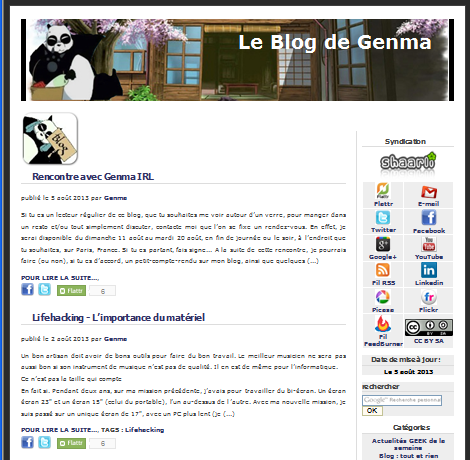
\includegraphics[width=5cm,height=5cm]{./images/blog.png} 
\end{columns}
\end{frame}


%------------------------------------------------
\begin{frame}
\frametitle{Programme}

\justifying{
Pourquoi ne dit-on pas crypter ? Un peu de théorie
\begin{itemize}
\item Le principe du chiffrement
\item Le chiffrement symétrique (Cesar)
\item Le chiffrement asymétrique (les enveloppes)
\end{itemize}
}


\justifying{
Le chiffrement en pratique
\begin{itemize}
\item Connexion Internet httpS
\item Le coffre-fort numérique avec TrueCrypt/Veracrypt
\end{itemize}
}

\justifying{
Comment est-on suivi à la trace sur Internet?
\begin{itemize}
\item Les publicités et le tracking par scripts (Le bouton j’aime de Facebook / Lightbeam)
\item Comment les bloquer.
\end{itemize}
}

\justifying{
Aller plus loin? Tor et le TorBrowser
\begin{itemize}
\item Comment l’installer, comment ça marche…
\end{itemize}
}

\end{frame}
%-----------------------------------------------
%-----------------------------------------------
\begin{frame}
\begin{center}
\Huge{Pourquoi ne dit-on pas crypter ? Un peu de théorie}
\end{center}
\end{frame}
%------------------------------------------------
\begin{frame}
\frametitle{XXXX}


\begin{block}{XXXX}
\justifying{
\begin{itemize}
\item 
\end{itemize}
}
\end{block}
\end{frame}
%-----------------------------------------------

%-----------------------------------------------
\begin{frame}
\begin{center}
\Huge{Le chiffrement en pratique}
\end{center}
\end{frame}
%------------------------------------------------
\begin{frame}
\frametitle{XXXX}


\begin{block}{XXXX}
\justifying{
\begin{itemize}
\item 
\end{itemize}
}
\end{block}
\end{frame}

%----------------------------------------------------------------------------------------
\begin{frame}
\frametitle{HttpsEverywhere}

Avoir une connexion httpS dès que possibe
\begin{center}
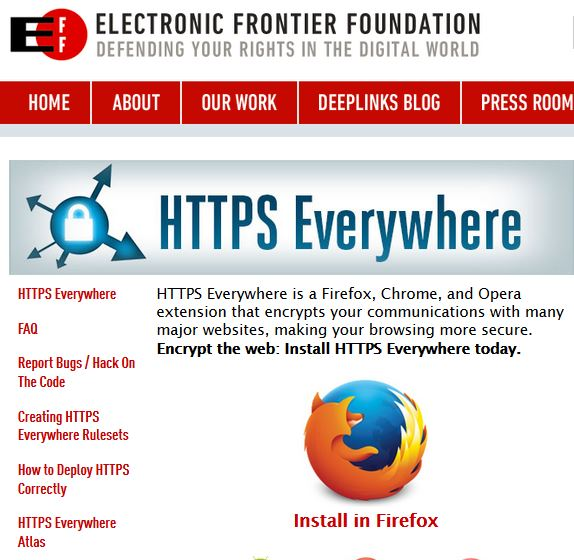
\includegraphics[scale=0.5] {./images/httpseverywhere.jpg}
\end{center}
\end{frame}
%-----------------------------------------------

%-----------------------------------------------
\begin{frame}
\begin{center}
\Huge{Comment est-on suivi à la trace sur Internet?}
\end{center}
\end{frame}

\begin{frame}
\frametitle{Comment est-on pisté ?}
\justifying{
\begin{block}{Toutes les publicités nous espionnent}
\begin{itemize}
\item Le bouton Like de Facebook : il permet à FaceBook de savoir que vous avez visité ce site, même si vous n'avez pas cliqué sur ce bouton.
\item Même si vous vous êtes correctement déconnecté de Facebook.
\item De même pour le bouton le +1 de Google, les scripts de Google Analytics, 
\item Tous les publicité, Amazon...
\end{itemize}
\end{block}
}
\begin{center}

\includegraphics[scale=0.3] {./images/Facebook_like.png}
\end{center}
\end{frame}

\begin{frame}
\frametitle{Le tracking publicitaire}
\begin{block}{Le pistage sur Internet}
\begin{itemize}
\justifying{
\item Le pistage est un terme qui comprend des méthodes aussi nombreuses et variées que les sites web, les annonceurs et d'autres utilisent pour connaître vos habitudes de navigation sur le Web. 
\item Cela comprend des informations sur les sites que vous visitez, les choses que vous aimez, n'aimez pas et achetez. 
\item Ils utilisent souvent ces données pour afficher des pubs, des produits ou services spécialement ciblés pour vous. 
}
\end{itemize}
\end{block}
\end{frame}

\begin{frame}
\frametitle{Lightbeam}
\begin{center}
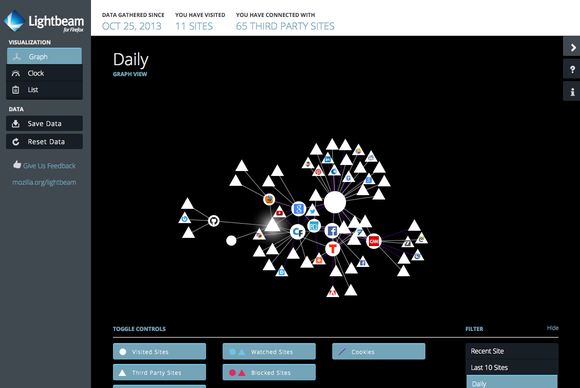
\includegraphics[scale=0.5] {./images/lightbeam.png}
\end{center}
\end{frame}

%----------------------------------------------------------------------------------------
\begin{frame}
\frametitle{AdBlock - block 1/2}
Page avec publicité :
\begin{center}
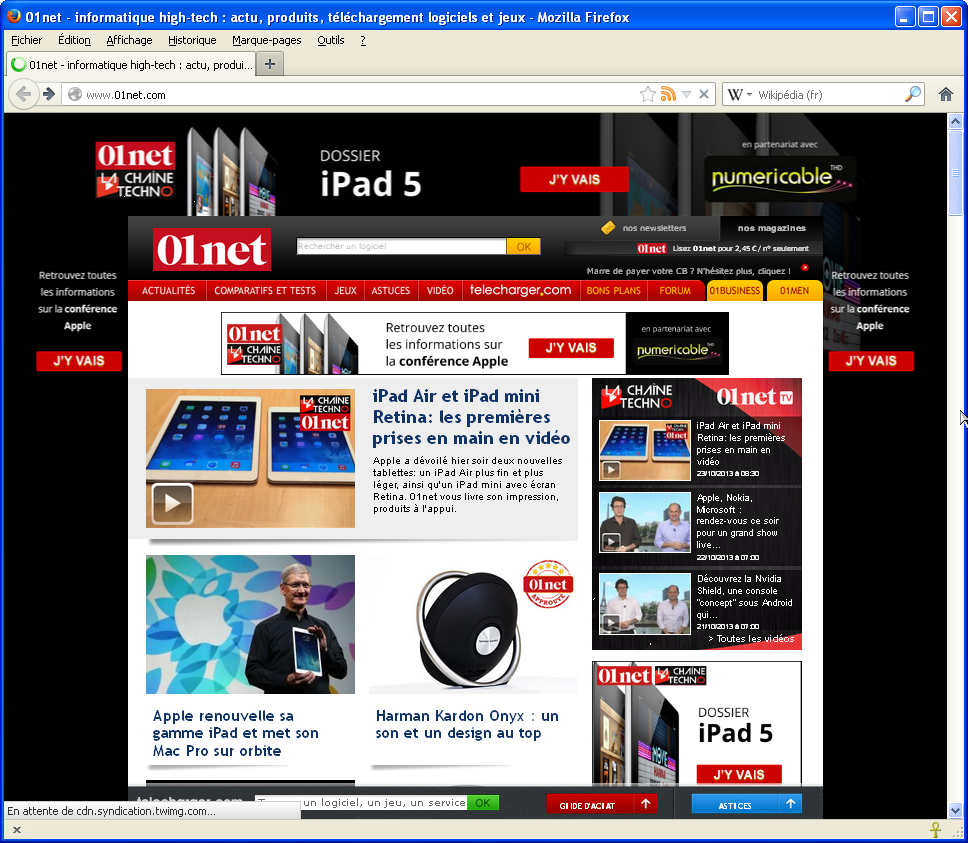
\includegraphics[scale=0.4] {./images/Adblock01.png}
\end{center}

\end{frame}

%----------------------------------------------------------------------------------------
\begin{frame}
\frametitle{AdBlock - Microblock 2/2}
Bloque les publicités. Allège les pages.

\begin{center}
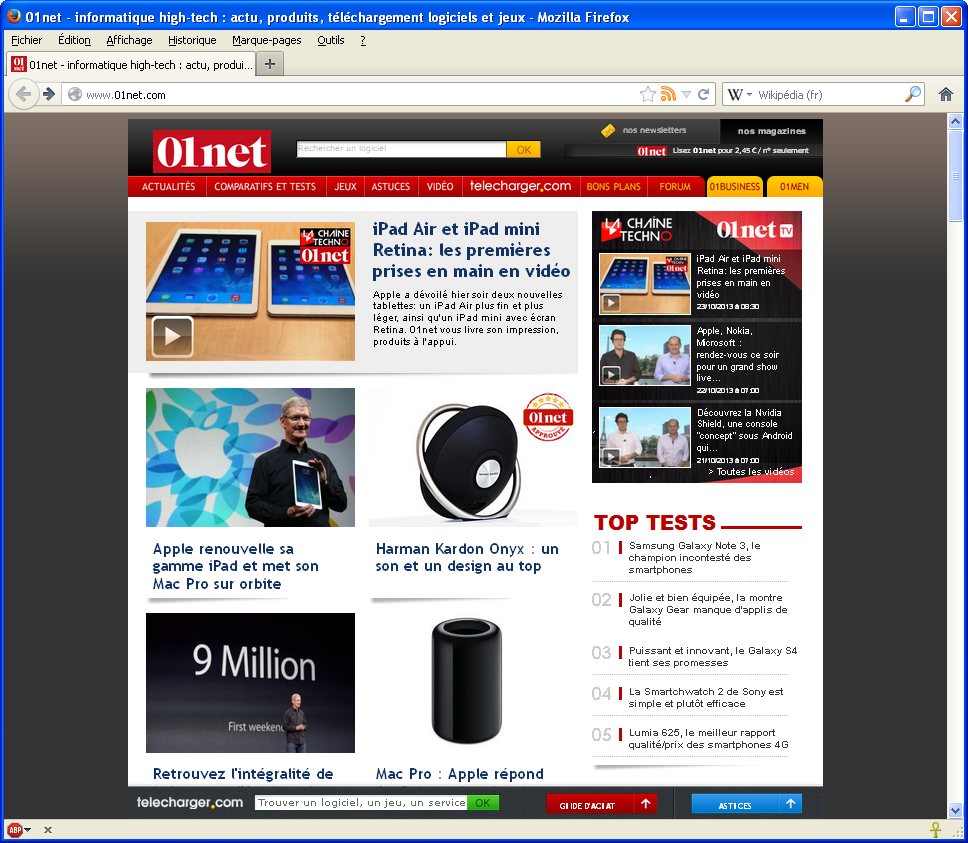
\includegraphics[scale=0.4] {./images/Adblock02.png}
\end{center}
\end{frame}

%----------------------------------------------------------------------------------------
\begin{frame}
\frametitle{Ghostery}

Bloque tous les trackers associés au site.
\begin{center}
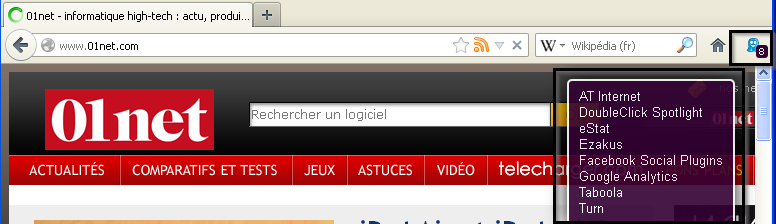
\includegraphics[scale=0.4] {./images/Ghostery_tracker.png}
\end{center}
\end{frame}



%-----------------------------------------------

%-----------------------------------------------
\begin{frame}
\begin{center}
\Huge{Aller plus loin? Tor et le TorBrowser}
\end{center}
\end{frame}


%----------------------------------------------------------------------------------------
\begin{frame}
\begin{center}
\Huge{Quelques mots sur Tor ? }
\\~\\ 
\includegraphics[scale=0.4]{./images/logo_tor.jpg}
\end{center}
\huge{Attention : la présentation \emph{complète} dure une bonne heure et demie...}
\end{frame}

%----------------------------------------------------------------------------------------
\begin{frame}
\frametitle{Comment fonctionne Tor ?}
\begin{center}
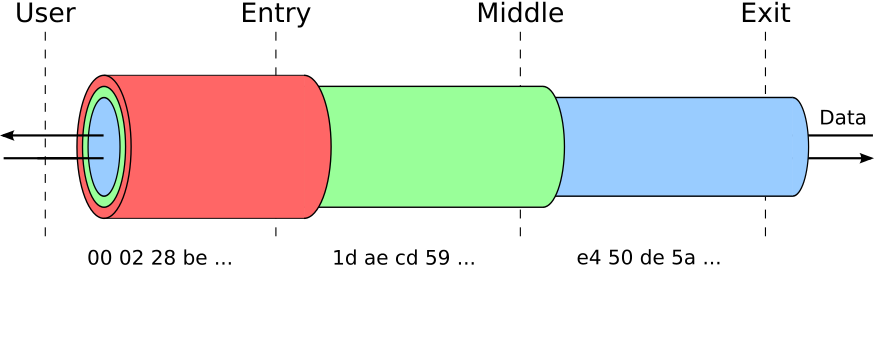
\includegraphics[keepaspectratio,width=\textwidth, height=.8\textheight]{images/tor-keys1}
\end{center}
\end{frame}

%----------------------------------------------------------------------------------------
\begin{frame}
\frametitle{A quoi sert TOR?}

\begin{block}{Ce que l'usage de Tor permet de faire}
\justifying{
\begin{itemize}
\justifying{
\item  d'échapper au fichage publicitaire,
\item  de publier des informations sous un pseudonyme,
\item  d'accéder à des informations en laissant moins de traces,
\item  de déjouer des dispositifs de filtrage (sur le réseau de son entreprise, de son Université, en Chine ou en France…),
\item  de communiquer en déjouant des dispositifs de surveillance,
\item  de tester son pare-feu,
\item  … et sûrement encore d'autres choses.
}
\end{itemize}
$\Rightarrow$ Tor dispose également d'un système de "services cachés" qui permet de fournir un service en cachant l'emplacement du serveur.
}
\end{block}
\end{frame}

%----------------------------------------------------------------------------------------
\begin{frame}
\frametitle{Télécharger le Tor Browser}
\justifying{
Toutes les versions (dans différentes langues, différents OS) sont disponibles sur le site du projet : 
\\ \url{https://www.torproject.org/}
\\ Rq : Il existe la possibilité de le recevoir par mail...
}
\begin{center}
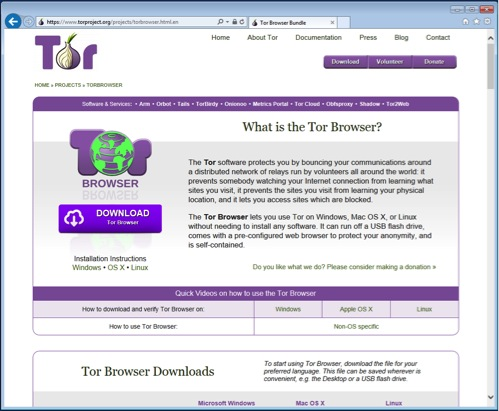
\includegraphics[scale=0.5]{./images/tor2.jpg}
\end{center}
\end{frame}

%----------------------------------------------------------------------------------------
\begin{frame}
\frametitle{Lancer le Tor Browser}
\begin{center}
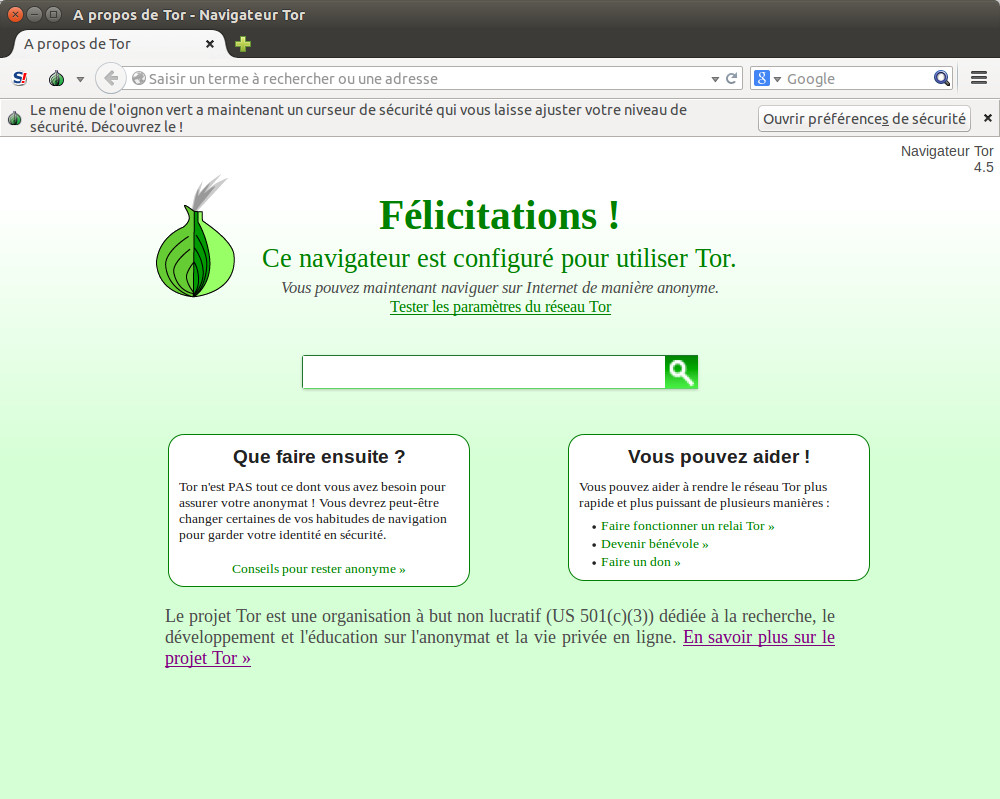
\includegraphics[scale=0.3]{./images/tor_browser03.jpg}
\end{center}
\end{frame}
%----------------------------------------------------------------------------------------

\begin{frame}
\frametitle{Utiliser Tor - Tails}
\justifying{
Tails (The Amnesic Incognito Live System) est un système d'exploitation complet basé sur Linux et Debian, en live.
}
\begin{center}
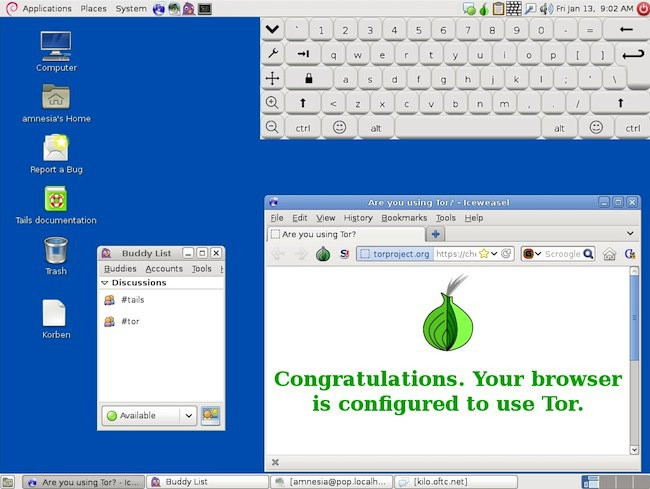
\includegraphics[scale=0.3]{./images/tails.jpg}
\\~\\
\url{https://tails.boom.org}
\end{center}
\end{frame}

%----------------------------------------------------------------------------------------
\begin{frame}
\Huge{\centerline{Merci de votre attention.}}
\Huge{\centerline{Place aux questions.}}
\end{frame}

%----------------------------------------------------------------------------------------
\begin{frame}
\frametitle{
\includegraphics[scale=0.4]{./images/Genma.jpg} \ \ \  Me contacter?}
\Huge{\centerline{Le Blog de Genma}}
\Huge{\centerline{http://genma.free.fr}}
\Huge{\centerline{~}}
\Huge{\centerline{Twitter : @genma}}
\end{frame}

%============================================================================================
\begin{frame}
\Huge{\centerline{ANNEXES}}
\end{frame}

%----------------------------------------------------------------------------------------
\begin{frame}
\frametitle{La navigation en mode privée 1/2}

\justifying{
\begin{block}{Quelles données ne sont pas enregistrées durant la navigation privée ?}
\begin{itemize}
\item pages visitées ;
\item saisies dans les formulaires et la barre de recherche ;
\item mots de passe ; 
\item liste des téléchargements ; 
\item cookies ;
\item fichiers temporaires ou tampons.
\end{itemize}
\end{block}
}
\end{frame}

%----------------------------------------------------------------------------------------
\begin{frame}
\frametitle{La navigation en mode privée 2/2}
\begin{center}
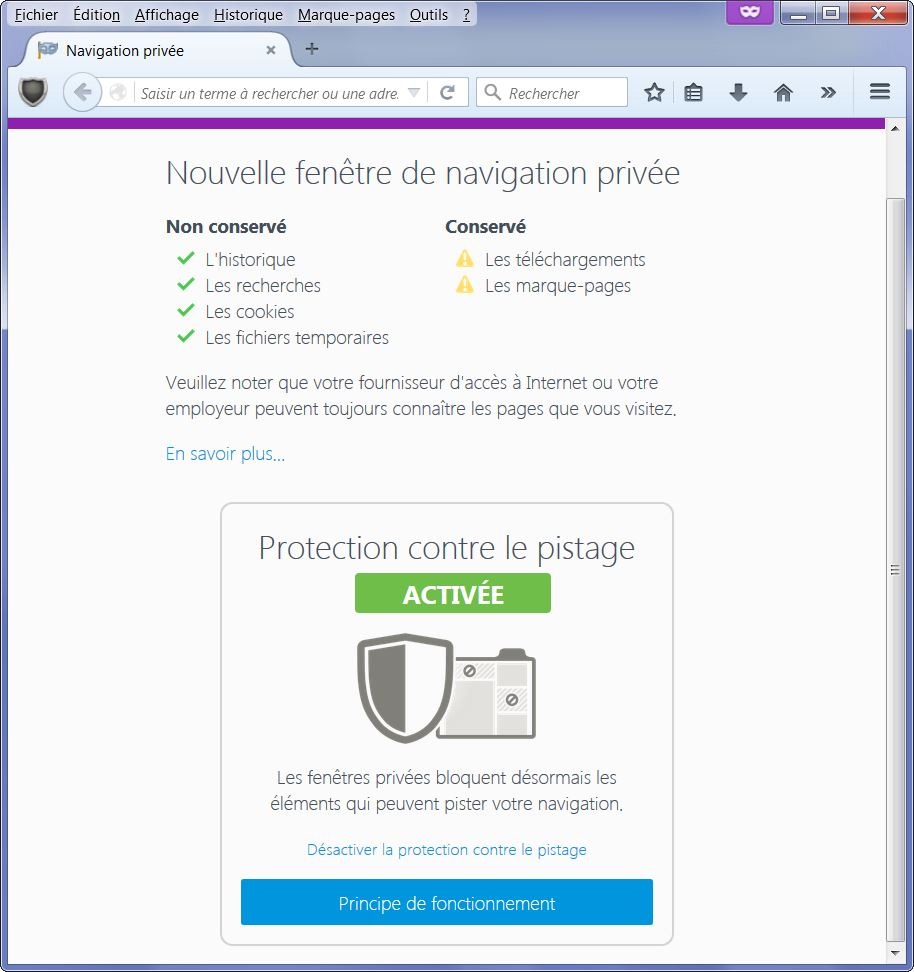
\includegraphics[scale=0.5] {./images/Navigation_privee.jpg} 
\end{center}
\end{frame}

%------------------------------------------------
\begin{frame}
\frametitle{Comment vérifier rapidement la sécurité d'un site ?}
\begin{block}{La check-liste}
\begin{itemize}
\justifying{
\item Le site a-t-il une connexion en https ? (SSL).
\item Y-a-t-il intégration d'éléments extérieurs au site en lui-même ?
\item Le site utilise-t-il Google Analytics ?
\item Le site utilise-t-il Google Fonts ?
\item Le site utilise-t-il des régies publicitaires ?
\item Le site utilise-t-il Cloudflare ?
\item Le DNS est-il géré par Cloudflare ?
\item Le site présente-t-il une politique de confidentialité ?
\item Le site utilise-t-il les cookies ?
\item Le site utilise-t-il des scripts javascript ?
}
\end{itemize}
\end{block}
\end{frame}

%----------------------------------------------------------------------------------------
\begin{frame}
\frametitle{Certificate Patrol}
Permet de valider les certificats d'un site (lié à https).
\begin{center}
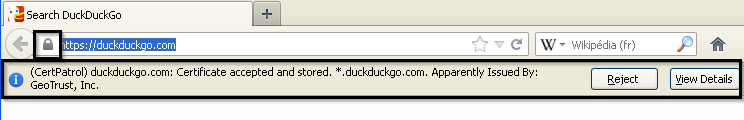
\includegraphics[scale=0.5] {./images/CertificatePatrol.png}
\end{center}
\end{frame}

%----------------------------------------------------------------------------------------
\begin{frame}
\frametitle{Certificate Patrol}
\begin{center}
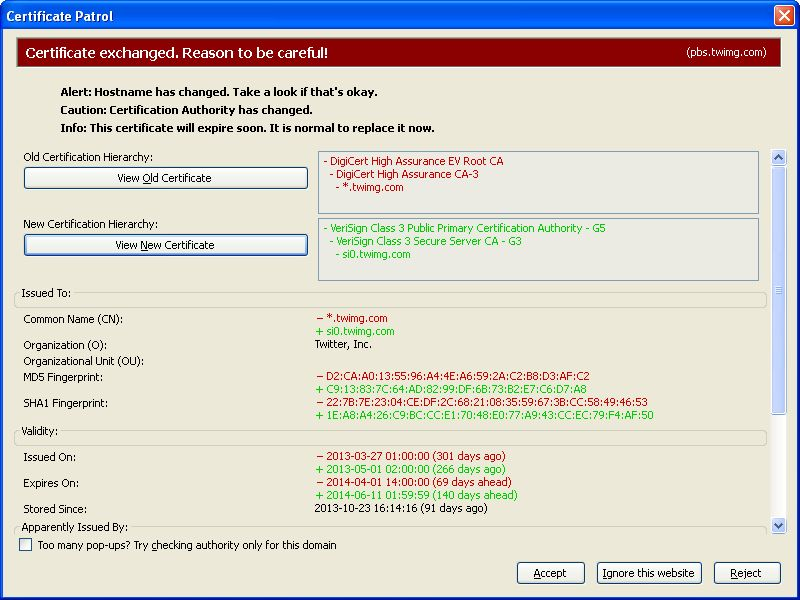
\includegraphics[scale=0.5] {./images/Certificate_Patrol_certifcat_a_change.jpg}
\end{center}
\end{frame}

%----------------------------------------------------------------------------------------
\begin{frame}
\frametitle{Calomel SSL}
\begin{center}
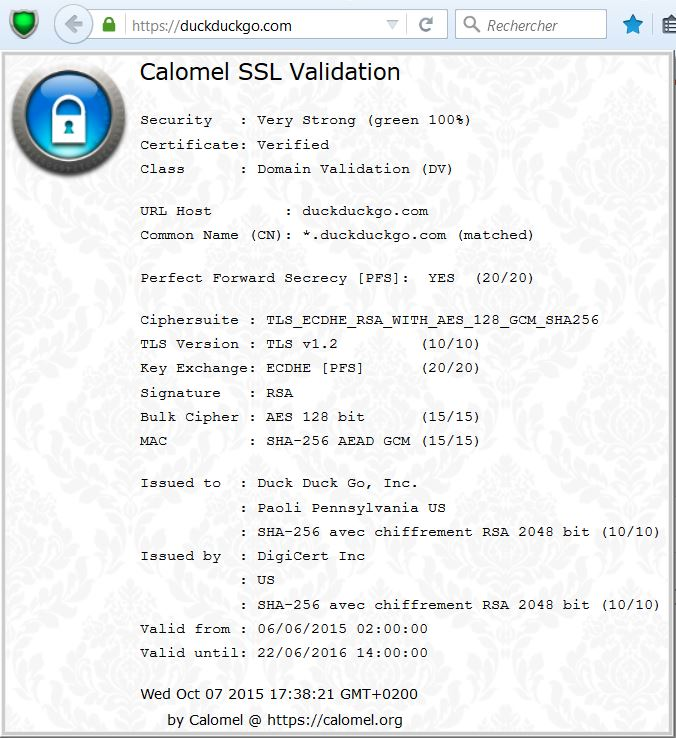
\includegraphics[scale=0.5] {./images/Calomel.jpg}
\end{center}
\end{frame}

%----------------------------------------------------------------------------------------
\begin{frame}
\Huge{\centerline{L'authentification forte}}
\end{frame}

\begin{frame}
\frametitle{L'authentification forte}

\begin{block}{Différents termes, un même usage}
Double authentification, Connexion en deux étapes, 2-Step Verification
\end{block}

\begin{block}{Exemple avec Google} 
\justifying{
Google permet aux utilisateurs d'utiliser un processus de vérification en deux étapes.
\begin{itemize}
\item La première étape consiste à se connecter en utilisant le nom d'utilisateur et mot de passe. Il s'agit d'une application du facteur de connaissance.
\item Au moment de la connexion Google envoit par SMS un nouveau code unique. Ce nombre doit être entré pour compléter le processus de connexion. 
\end{itemize}
Il y a aussi une application à installer qui génère un nouveau code toutes les 30 secondes.
}
\end{block}
\end{frame}

%----------------------------------------------------------------------------------------
\begin{frame}
\frametitle{L'authentification forte}
\begin{block}{Autres services implémentant cette fonctionnalité}
\begin{itemize}
\item Web : Facebook, Twitter, Linkedin, Paypal
\item Banque : envoit d'un code par SMS
\end{itemize}
\end{block}
\end{frame}


\end{document}